



\chapter{Jets in Proton-Proton Collisions}%\label{ch1:intro}



A jet is a collimated grouping of hadrons usually associated with the LO production of a parton, quark or gluon. In this case the quark (gluon) could be initiated by the hard scatter of 2 constituent partons from protons or be the decay product of another particle that was produced in the hard scatter, such as a W boson, which can then decay to 2 quarks each forming a jet. The initial parton radiates other quarks and gluons, called the "Parton Shower" and all color charged particles fragment into hadrons, mainly pions and kaons,  before reaching the detector as mentioned in ~\ref{chap:MCGenReco}.

Studies of jets at LHC are complicated by experimental complexities such as "underlying event", other partons from the same proton interacting and depositing energy in the same region of the detector. "Pileup" is also increasingly relevant, like "underlying event" but initiated from other proton interactions from this or a previous bunch, since the LHC crosses bunches with $~10^{11}$ protons every 25 nanoseconds.



Any measurement is limited by the resolution of the measurement device and any detector effect. In this thesis the results are disentangled from the reconstructed data by "unfolding" the reconstructed distributions back to generator level.

While jets are often used as simple proxies for the quark or gluon from which they originated, the structure of the radiation pattern of the hard scatter is encoded within the jet's constituent particles~\cite{Asquith:2018igt}. Jet studies are essential for a complete understanding of proton-proton interactions since the majority of interesting physics signatures contain a color charged parton in the final state. This chapter covers the basics of jet physics at LHC, from the algorithms used for clustering the constituent particles in experimental data to the language and calculations of the theory.

% cite https://arxiv.org/pdf/1901.10342.pdf simones book



\section{Jet Clustering Algorithms}\label{secSM:ch1}

At LO, a jet represents a quark [gluon], however realistically that is not a well defined concept and a more precise definition is useful. This thesis adopts the definition presented at the Les Houghes conference in 2015 :\newline

"A phase space region (as defined by an unambiguous hadronic fiducial cross section measurement) that yields an enriched sample of quarks [gluons] (as interpreted by some suitable, though fundamentally ambiguous, criterion)"~\cite{Badger:2016bpw}.\newline 

I will discuss one class of "suitable, though fundamentally ambiguous" criteria for defining jets, known as sequential recombination algorithms. These algorithms take pairs of particles and successively combine them into 1 particle, in a way which is intended to reconstruct the successive branchings of partons within the jet as described by perturbative QCD ~\cite{Marzani:2019hun}.
 
% rivello: Broken citation at the paragraph below:
In sequential recombination algorithms a distance metric, $d_{ij}$, is defined between all particle pairs. These pairs are then sequentially combined in order of increasing distance. Three popular algorithms in this class can be described by the equation ~\cite{eq:sequRec}:


\begin{equation}\label{eq:sequRec}
\begin{array}{l}{d_{i j}=\min \left(p_{t i}^{2 p}, p_{t j}^{2 p}\right) \frac{\Delta R_{i j}^{2}}{R^{2}} \quad \Delta R_{i j}^{2}=\left(y_{i}-y_{j}\right)^{2}+\left(\phi_{i}-\phi_{j}\right)^{2}} \\ {d_{i B}=p_{t i}^{2 p}}\end{array}
\end{equation}


Depending on the value chosen for $p$, this equation can produce a variety of clusterings, herein I discuss the 3 popular choices $p = [1, 0, -1]$ refering to them by their names: KT ~\cite{Ellis:1993tq}, Cambridge/Aachen ~\cite{Dokshitzer:1997in} and Anti\kt algorithms ~\cite{Cacciari:2008gp} respectively.

Each algorithm has its own specific use cases and drawbacks. For example, the Anti\kt algorithm produces circular jets of constant area as seen in ~\ref{fig:antikt}. 

\begin{figure}[htb]
\centering
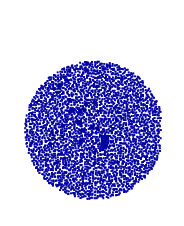
\includegraphics[width=.40\textwidth]{visuals/figs_subjet-plots-antikt.png}
\caption{For jets clustered using the Anti\kt algorithm a circular pattern emerges, making pileup and underlying event subtraction simpler for experimentalists~\cite{Dreyer:2018nbf}.}
\label{fig:antikt}
\end{figure}



This constant area is useful for experimental studies as it allows for simple removal of underlying event energy, which is evenly distributed throughout the jet area ~\cite{Dreyer:2018nbf}. In contrast to the other 2 algorithms described, the C/A algorithm does not contain any momentum weighting, this leads to jets which are not circular, depicted in ~\ref{fig:cashape}, and instead follow the radiation pattern of the original jet constituent particles as seen in ~\ref{fig:cashape}. The variation in the way these algorithms cluster the underlying radiation is depicted in ~\ref{fig:algclusterdiffs}. In this thesis we have chosen to recluster the Anti\kt jets with C/A in order to preserve the original radiation pattern.


%##image C/A vs anti-Kt --- visuals/config-antikt-double-lund
\begin{figure}[htb]
\centering
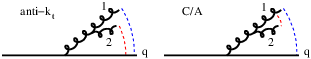
\includegraphics[width=1.0\textwidth]{visuals/config-antikt-double-lund.png}
\caption{Notice that the clustering follows the radiation pattern for C/A while the softer emissions are clustered with the jet axis in the case of Anti\kt ~\cite{Dreyer:2018nbf}.}
\label{fig:algclusterdiffs}
\end{figure}


\begin{figure}[htb]
\centering
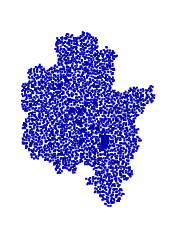
\includegraphics[width=.40\textwidth]{visuals/figs_subjet-plots-CA.png}
\caption{Jets clustered using C/A algorithm are not circular, instead they are shaped like the radiation pattern~\cite{Dreyer:2018nbf}.}
\label{fig:cashape}
\end{figure}


% good section on it here
% http://inspirehep.net/record/1123042/files/fermilab-thesis-2012-12.pdf

%# https://arxiv.org/pdf/1304.1025.pdf
%Sequential recombination algorithm for jet clustering and








%#

%#


\section{Jet Grooming}\label{sec:jetgroom}

Jet grooming is a broad term to describe a number of different algorithms intended to remove some portion of the soft and collinear radiation within a jet. This analysis uses the Soft-Drop (SD) algorithm~\cite{softdrop} which removes soft and collinear radiation in a theoretically controlled manner. The SD procedure is as follows: Begin with an Anti\kt ~\cite{Cacciari:2008gp} clustered jet composed of particle flow candidates, reclustered with Cambridge-Aachen algorithm~\cite{Dokshitzer:1997in} to remove the \pt weighting dependance of the clustering. At this stage we regress through the clustering history, keeping a subjet if it meets of SD criterion and otherwise "dropping" it.

% FIX ME ref particle flow section

SD iteratively declusters a jet $j$ with distance parameter $R$ into two subjets, $j_1$ and $j_2$.
If the softdrop condition

\begin{equation}
  \frac{\min(p_{T1},p_{T2})}{p_{T1}+p_{T2}} > z_{cut} \cdot (\frac{\Delta R_{12}}{R})^\beta
\end{equation}

is met, then the procedure terminates and $j$ is the final state jet. Otherwise, the declustering continues - 
the higher $\pt$ subjet is relabeled as $j$ and the lower $\pt$ ("softer") subjet is dropped, hence the name.
By design, this condition fails for wide-angle soft radiation, which is therefore removed by the soft
drop procedure. The tunable parameters, $\beta$ and $z_{cut}$, control the degree of jet grooming:
$\beta$ tunes the algorithm's sensitivity to wide-angle radiation, while $z_{cut}$ sets the energy scale
of the grooming. In the case of $\beta \rightarrow \infty$, an ungroomed jet is returned. 
In the $\beta = 0$ case, the soft drop procedure is identical to the ``modified mass drop tagger'' (MMDT)
from Ref.~\cite{mmdt}. For $\beta > 0$  soft emissions are removed from the jet while the majority of the collinear emissions remain, as illustrated in ~\ref{fig:softdroplund}. 


\begin{figure}[htb]
\centering
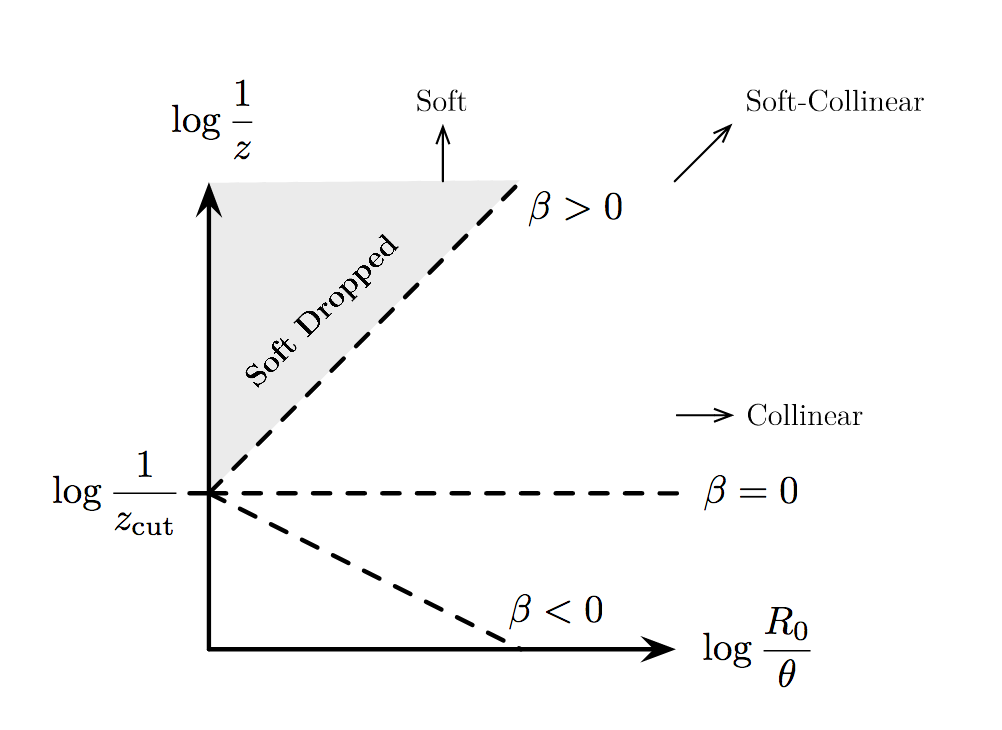
\includegraphics[width=1.0\textwidth]{visuals/softdroplund.png}
\caption{An illustration of the phase space for jet emissions outlining which would be groomed away by the SD procedure ~\cite{softdrop}.}
\label{fig:softdroplund}
\end{figure}
%#

The soft drop algorithm removes soft and wide-angle radiation
from jets in a very theoretically controlled manner, making it suitable to separate
the ``hard'' and ``soft'' parts of the jet. Specifically, the soft drop
algorithm can remove non-global logarithms from correlations of
radiation within and between jets, which are extremely difficult to
compute theoretically~\cite{Dasgupta:2001sh,mmdt,softdrop,Dasgupta:2013via,Dasgupta:2015yua,Larkoski:2015zka}.



%Casimir Meets Poisson: Improved Quark/Gluon Discrimination with Counting Observables
%https://arxiv.org/abs/1704.06266
%soft drop multiplicity







%%%%%%%%%%%%%%%%% Lund Jet Plane



\section{Lund Jet Plane}\label{sec:lundjetplane}


   ~\ref{fig:introlund}




\begin{figure}[htb]
\centering
\includegraphics[width=.90\textwidth]{visuals/introlund.png}
\caption{A Lund kinematic Diagram is composed of }
\label{fig:introlund}
\end{figure}






%%%%%%%%%%%%%%%%% Jet Mass section



\section{Jet Mass}\label{sec:jetmass}


Jet mass is a simple observable, useful for probing QCD. The calculations for the jet mass at leading order are described below for the plain and soft-drop groomed jets.

\subsection{Plain Jet Mass}\label{sec:jetmass}


In this section quark jet mass calculations are discussed at LO. 




\begin{figure}[htb]
\centering
\includegraphics[width=1.10\textwidth]{visuals/quarkGluonPlainvsGroomedMass.png}
\caption{(Left) The distribution of $\rho$ for tagged jets, with three taggers/groomers: pruning , trimming and the mass-drop tagger (MDT). The results have been obtained from Monte Carlo simulation with \PYTHIA 6.425~\cite{Sjostrand:2014zea}, for 14 TeV proton-proton collisions, at parton level, including initial and final-state showering, but without the underlying event (multiple interactions). (Right) Analogous distribution for Gluon jets.~\cite{mmdt}}
\label{fig:quarkGluonPlainvsGroomedMass}
\end{figure}




















Higher order corrections to the hard process are nessessary in order to properly predict measurements in the non-perturbative regime. This can be seen clearly in the dijet dimensionless mass spectrum measured by the ATLAS collaboration (Maybe replace with our result but I am not sure which plot to use as ours seem to agree even at low mass[presumably bc we only showed the more accurate predictions by Marzani and Frye rather than all of the others] ) ~\ref{fig:atlasDijet}


\begin{figure}[htb]
\centering
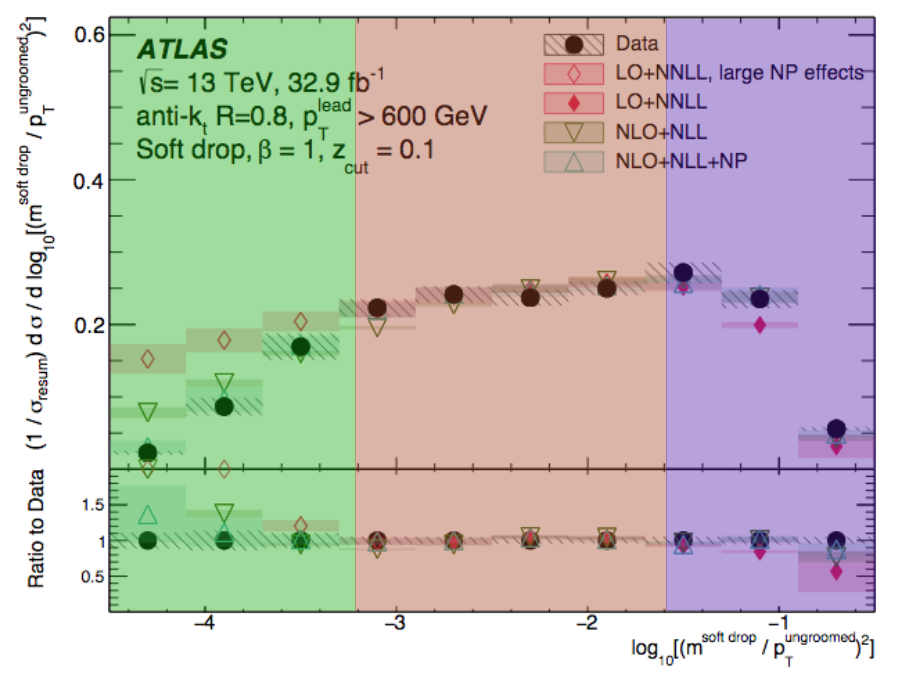
\includegraphics[width=.60\textwidth]{visuals/ATLAS-rho-highorder.png}
\caption{Above is the ATLAS Dijets dimensionless mass result ~\cite{Dreyer:2018nbf}.Next to Leading Order + Next to Leading Log + NonPerturbative corrections were required in order to match data in non-perturbative regime (Far left of this plot, shaded green column).}
\label{fig:atlasDijet}
\end{figure}







% pilup images with diff algorithms
%# https://arxiv.org/pdf/1304.1025.pdf
%Sequential recombination algorithm for jet clustering and

%Towards Jetography
%Gavin P. Salam
%$https://arxiv.org/abs/0906.1833
\cite{Salam:2009jx}

\cite{Asquith:2018igt}
%https://arxiv.org/pdf/1803.06991.pdf
%Jet Substructure at the Large HadronCollider :  Experimental Review



% DY thesis https://cds.cern.ch/record/2018454/files/CERN-THESIS-2015-048.pdf
\section{Jet Production Cross Sections}\label{sec:jetProdCrossSections}

Jets are produced copiously at LHC and are involved in the final states signal and background of many interesting processes. 


\begin{equation}
\sigma=\sum_{a, b} \int_{0}^{1} d x_{a} d x_{b} \int d \Phi_{n} f_{a}^{h_{1}}\left(x_{a}, \mu_{F}\right) f_{b}^{h_{2}}\left(x_{b}, \mu_{F}\right) \frac{1}{2 \hat{s}}\left|\mathcal{M}_{a b \rightarrow n}\right|^{2}\left(\Phi_{n} ; \mu_{F}, \mu_{R}\right)
\end{equation}

The normalized differential cross section is measured in this analysis as described in ~\ref{sec:intro}

